%!TEX root = ../../secondYearReport.tex

\subparagraph{System dynamics estimation software. Extension to
environmental compliance estimation (T1.4)}

The goal of this task is to develop a software tool for on-line identification
of whole-body dynamics, as well as the compliance of contacts established
between the robot and the environment.

\begin{itemize}
\item Within T1.4, IIT continued the activities started during the previous
  year, with specific focus on whole-body identification \cite{Traversaro2013,
    Traversaro2014}.  In order to enhance the identification accuracy, an
  in-situ force/torque sensor calibration procedure was designed
  \cite{Traversaro2015b} (see Fig.~\ref{fig:validation}) and implemented in a
  software
  component\footnote{\url{https://github.com/robotology-playground/insitu-ft-calibration}.}
  which has been released with an open source license.  Similarly, in order to
  enhance the torque estimation accuracy, IIT conducted a theoretical analysis
  that exploits embedded force/torque sensors.  It has been proven
  \cite{Traversaro2015} that the inertial parameters estimated from embedded
  force/torque sensors can be successfully used for torque estimation.
\item During year two, TUD worked with the WBI toolbox in Matlab to study
  whole-body controllers capable of integrating learned inverse dynamics
  models.  The idea, more specifically, is to combine the low-level torque
  control at joint level with the learned dynamics models of WP4 (T4.2), which
  can thus provide the correct torques for rigid and compliant contacts.  TUD
  implemented a whole-body impedance controller and two balance controllers
  with the WBI toolbox in Matlab (see Figure~\ref{fig:wbitud}).  The
  controllers were tested on Gazebo and on the iCub mex model simulated in
  Matlab.  The integration with the outcome of WP4 is ongoing.
\end{itemize}

\begin{figure}[h]
\vspace{0.5em}
\centering
{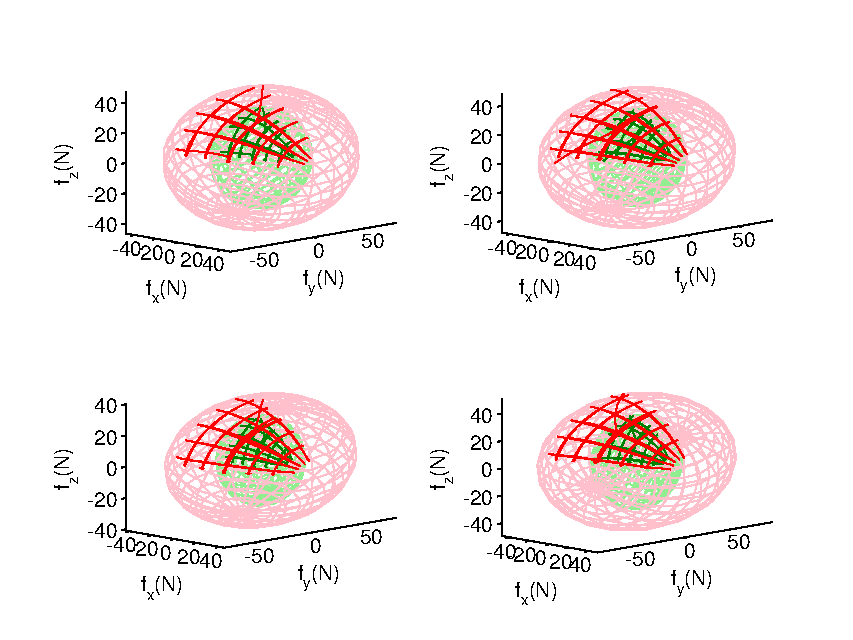
\includegraphics[width=0.65\textwidth]{images/leg_validation.pdf}}
\caption{The image shows the accuracy in calibrating the force/torque sensor
  with the procedure described in \cite{Traversaro2015b}. The four plots refer
  to four different experimental conditions (different values for the
  calibration weights).  Ideally, perfectly calibrated data should lie on the
  surface of a three dimensional sphere. Dark green: force measurements
  obtained with the calibration matrix estimated using the proposed
  technique. Dark red: force measurements obtained with the calibration matrix
  provided with the sensor.  Light red and light green surfaces: ellipsoids
  fitted to the measured forces.  Qualitative calibration accuracy can be
  obtained by looking at the spherical symmetry of the fitted ellipsoids.}
\label{fig:validation}
\end{figure}

 \begin{figure}
 \centering
 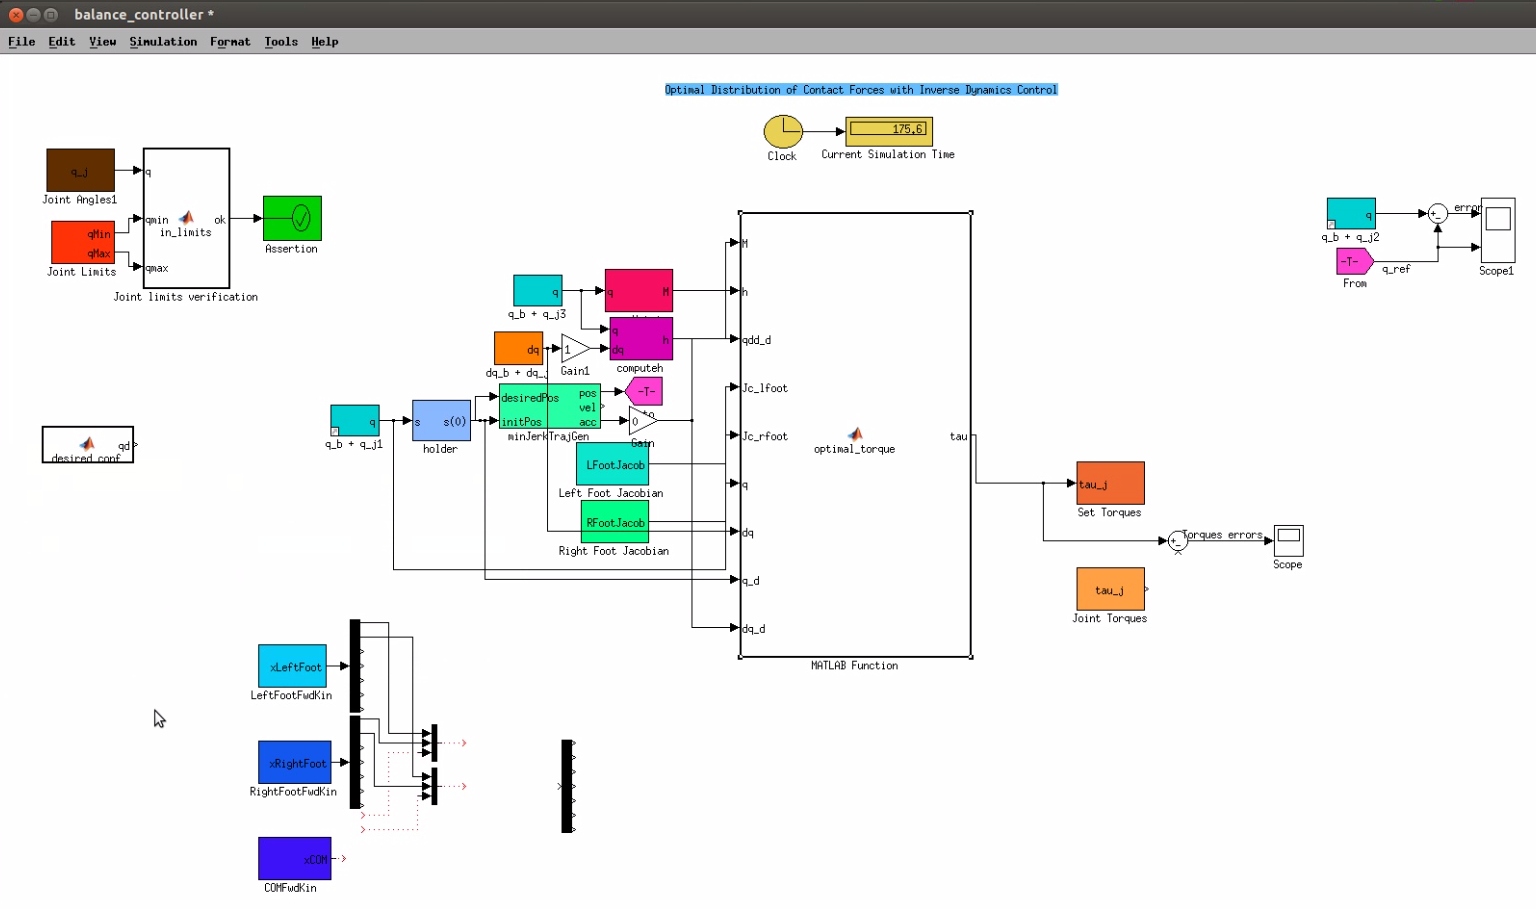
\includegraphics[width=0.7\textwidth]{wbi_torque_controller.png}
  \caption{One of the balance controllers implemented by TUD with the WBI
    toolbox in Matlab.  }
 \label{fig:wbitud}
 \end{figure}
